\subsection*{What is a Plasma?}
    \line

    \begin{definition}[Plasma]
        ``Plasma'' refers here to an electrically charged fluid, typically occurring when a fluid is supplied with sufficient energy—from heating or an applied electromagnetic (EM) field—that a significant portion of the atoms \BA{(Not molecules?)} are ionised \BA{(Terminology?)}, causing the (positive) ion and (negative) electron phases to move independently.
    \end{definition}
    
    \line

    Plasma is one of the most abundant forms of matter in the universe \cite{CL13}, found most frequently in stars \cite{Phi95, Asc06, Pie17} and similarly—as in our case—the star-like environments emulated in a tokamak.
    
    While an applied EM field induces a current as it separates the two charged phases: the ions and electrons, the current similarly induces and EM field through Maxwell's equations, creating a complex, coupled, nonlinear system. \BA{[Ref.]}
    \begin{center}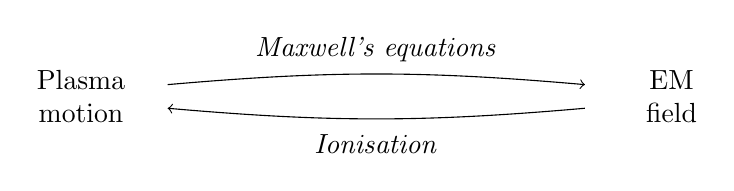
\begin{tikzpicture}[align = center, node distance = 4cm, auto]
        \node (1) at (0, 0) {Plasma \\ motion};
        \node (2) at (7.5, 0) {EM \\ field};
        
        \draw[->] (1.1, 0.15) to [out = 5, in = 175] (6.4, 0.15);
        \node at (3.75, 0.6) {\emph{Maxwell's equations}};
        \draw[->] (6.4, -0.15) to [out = 185, in = -5] (1.1, -0.15);
        \node at (3.75, -0.6) {\emph{Ionisation}};
    \end{tikzpicture}\end{center}
    